\documentclass{article}
\usepackage[utf8]{inputenc}
\usepackage[margin=1in]{geometry}

 
\usepackage{listings}
\usepackage{color}
\usepackage{graphicx}
\usepackage{float}
\usepackage{amsmath}
 
\definecolor{codegreen}{rgb}{0,0.6,0}
\definecolor{codegray}{rgb}{0.5,0.5,0.5}
\definecolor{codepurple}{rgb}{0.58,0,0.82}
\definecolor{backcolour}{rgb}{0.95,0.95,0.92}
 
\lstdefinestyle{mystyle}{
    backgroundcolor=\color{backcolour},   
    commentstyle=\color{codegreen},
    keywordstyle=\color{magenta},
    numberstyle=\tiny\color{codegray},
    stringstyle=\color{codepurple},
    basicstyle=\footnotesize,
    breakatwhitespace=false,         
    breaklines=true,                 
    captionpos=b,                    
    keepspaces=true,                 
    numbers=left,                    
    numbersep=5pt,                  
    showspaces=false,                
    showstringspaces=false,
    showtabs=false,                  
    tabsize=2
}
 
\lstset{style=mystyle}

\newcommand*{\mybox}[1]{\framebox{\strut #1}}

 

\title{CSC 583 Homework 3}
\author{Sina Ehsani}
\date{\today}



\begin{document}
\maketitle


\section{Problem 2}



\textbf{Compute variable byte codes and $\gamma$ codes for the postings list $< 777, 17743, 294068, 31251336 >$. Use gaps instead of docIDs where possible. Write binary codes in 8-bit blocks. You can use Google, or any other resource, to convert numbers to binary.}
\\
First we transfer the posting lists to gaps (as follows):
$< 777, 16966, 276325, 30957268 >$
Then for each number we have following:
\\
\\
\begin{tabular}{ |c|c|c|c| } 
\hline
 Posting(gaps) & Binary & VB  \\ 
 \hline
 777 & 1100001001 & 00000110 10001001\\ 
 16966 & 100001001000110 & 00000001 10000100 11000110 \\ 
 276325 & 1000011011101100101 & 00010000 11101110 11100101\\ 
 30957268 & 1110110000101111011010100 & 00001110 11100001 10111101 11010100 \\ 
 \hline
\end{tabular}
\\
\\
\\
\begin{tabular}{ |c|c|c| } 
\hline
 Posting(gaps) & offset & Gamma \\ 
 \hline
 777 & 100001001 & 1111111110,100001001\\ 
 16966 & 00001001000110 & 111111111111110,00001001000110\\ 
 276325 & 000011011101100101 & 1111111111111111110,000011011101100101\\ 
 30957268 & 110110000101111011010100 & 1111111111111111111110,110110000101111011010100\\ 
 \hline
\end{tabular}

\pagebreak


%\begin{figure}[H]
%\begin{center}
%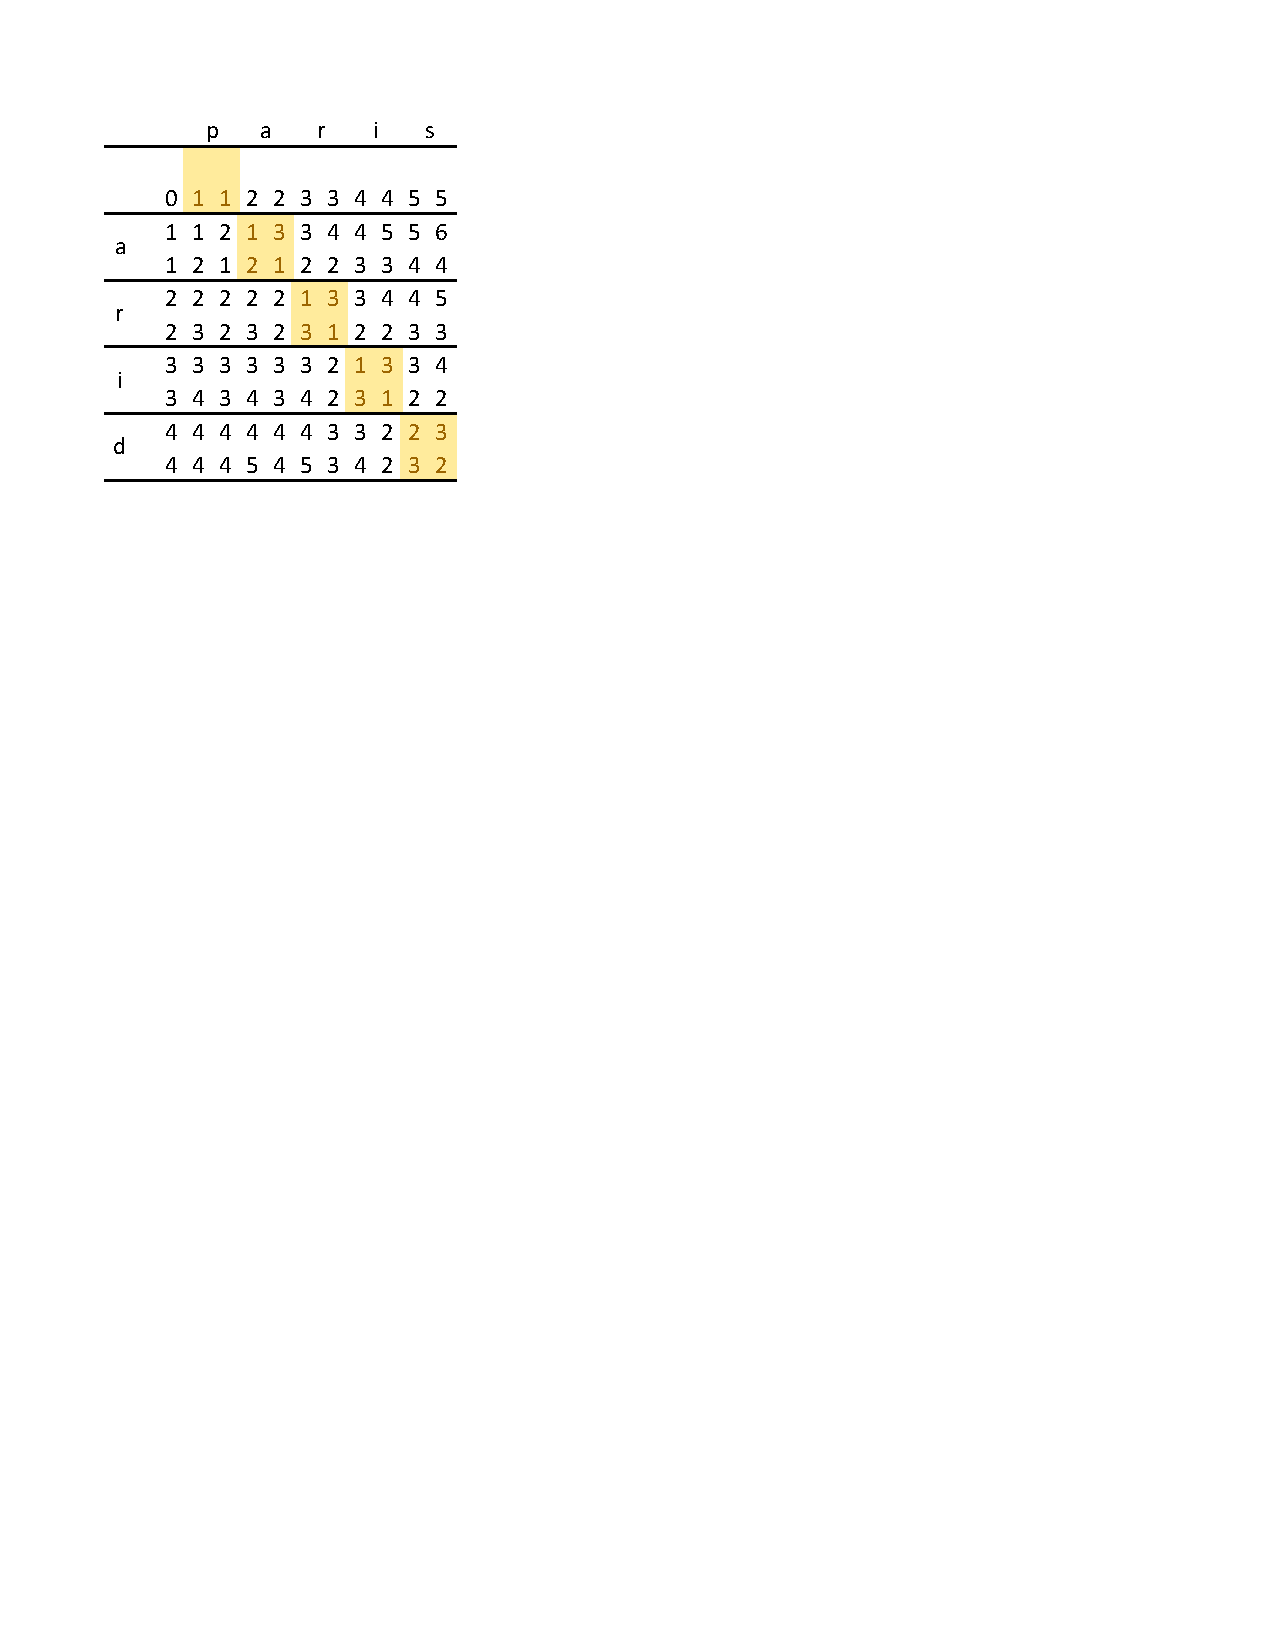
\includegraphics[width=3in]{Workbook1.pdf}
%\caption{The yellow path shows the minimum edit distance path}
%\label{distmatrix}
%\end{center}
%\end{figure}

\section{Problem 3}

\textbf{From the following sequence of $\gamma$-coded gaps, reconstruct first the gap sequence and then the postings sequence: $1110001 11010 101 11111011011 11011$.}
\\
\\
\begin{tabular}{ c|c|c|c } 

 Gamma & binary & gaps & postings \\ 
 \hline
 1110,001 & 1001 & 9 & 9\\ 
 110,10 & 110 & 6 & 15\\ 
 10,1 & 11 & 3 & 18\\ 
 111110,11011 & 111011 & 59 & 77\\ 
 110,11 & 111 & 7 & 84\\ 

\end{tabular}

\pagebreak

\section{Problem 4}

\textbf{Consider the table of term frequencies for 3 documents denoted Doc1, Doc2, Doc3 in the table below (in assignment). Compute the tf-idf weights for the terms “car”, “auto”, “insurance”, and “best”, for each document, using the idf values from the second table.}
\\
\\
\begin{tabular}{lc|ccc|ccc|ccc}
                               &      & \multicolumn{3}{c|}{DOC1} & \multicolumn{3}{c|}{DOC2} & \multicolumn{3}{c}{DOC3} \\ \hline
\multicolumn{1}{l|}{Word}      & idf  & tf  & tf-weight  & tf-idf & tf  & tf-weight  & tf-idf & tf & tf-weight & tf-idef \\ \hline
\multicolumn{1}{l|}{car}       & 1.65 & 27  & 2.43       & 4      & 4   & 1.6        & 2.6    & 24 & 2.38      & 3.9     \\
\multicolumn{1}{l|}{auto}      & 2.08 & 3   & 1.47       & 3      & 33  & 2.5        & 5.2    & 0  & 0         & 0       \\
\multicolumn{1}{l|}{insurance} & 1.62 & 0   & 0          & 0      & 33  & 2.5        & 4      & 29 & 2.46      & 4       \\
\multicolumn{1}{l|}{best}      & 1.5  & 14  & 2.15       & 3.2    & 0   & 0          & 0      & 17 & 2.23      & 3.3    
\end{tabular}

\pagebreak


\section{Problem 5}

\textbf{1. What is the idf of a term that occurs in every document? Compare this with the use of stop word lists.}

$$ df=n \Rightarrow \log \frac{N}{N} = log1 = 0 $$
the $df$ will be equal to $N$ (number of documents), and the log will be 0. So the term would not have any weight in the tf-idf. This will help the search result in the way that the frequent stop words (i.e. the) have very small value in the tf-idef weight. 
\\
\\
\textbf{2. How does the base of the logarithm in the idf formula affect the score calculation of the following formula:}
$$Score(q, d) = \sum tf.idf_{t,d}$$
\textbf{Does a different logarithm base affect the relative scores of two documents on a given query? If so, how? To answer this question, you must know how to change the base of a logarithm. Google “how to change the base of a logarithm” :)}
\\\\
Lets see the effect with an example: we are searching "car insurance" for two documents with fixed tf scores. If number of total document is 10000 and we have the term "car" that is in 100 of these documents, and term "insurance" that exists in only 10. Then we have the following values of idf for different bases:

\begin{center}

\begin{tabular}{ c|c|c|c|c|c|c } 

 & df & 10 & 2 & 5 & 20 & 100 \\ 
 \hline
 car  & 100 & 2  & 6.64 & 2.86  & 1.53 & 1\\ 
 insurance & 10 & 3 & 9.96 & 4.29 &  2.3 & 1.5\\ 
 
 \end{tabular}
\end{center}

As you can see from the above the table, the difference between the importance of the more frequent term (car) and the less frequent term (insurance) will reduce when increasing the bias. In the other hand by decreasing the bias we give more importance to low frequency terms.  

\pagebreak


%\lstinputlisting[language=Python]{q7p1.py}

\end{document}

